\documentclass[12pt]{article}
\usepackage[top=1cm, bottom=3cm, right=2cm, left=2cm]{geometry}
\usepackage{amsfonts, amssymb, amsmath, hyperref}
\usepackage{graphicx}
\usepackage[T1, T2A]{fontenc}% T2A for Cyrillic font encoding
\usepackage[english, russian]{babel}
\usepackage[justification=centering]{caption}
\usepackage{wrapfig,lipsum,booktabs}
\usepackage{placeins}
\usepackage{subcaption}
\usepackage{multirow}
\usepackage{indentfirst}

\begin{document}
\title{\textbf{Лабораторная работа 3.3.4}\\ [4pt]{Эффект Холла в полупроводниках}}
\date{\today}
\author{Татаурова Юлия Романовна}

\begin{document}
\maketitle
\textbf{Цель работы:} измерение подвижности и концентрации носителей заряда
в полупроводниках.\\\indent
\textbf{Оборудование:} электромагнит с источником питания, батарейка, амперметр, реостат, цифровой вольтметр, милливеберметр, образец легированного германия.

\section*{Теоретические сведения}
\indent Во внешнем магнитном поле $B$ на заряды действует сила Лоренца, которая вызывает движение носителей заряда. При этом траектория частиц будет искривляться, поэтому будет возникать разность потенциалов в направлении поперечном току в образце. В этом и заключается эффектт Холла.
\section*{Экспериментальная установка}

\indent В зазоре электромагнита создается постоянное магнитное поле, которое можно менять с помощью регуляторов источника питания. 
Ток измеряется амперметром источника питания $A_1$.\\
\indent При замыкании ключа $K_2$ вдоль длинной стороны образца течет ток, величина которого изменяется реостатом $R$ и измеряется миллиамперметром $A_2$.\\
\indent В образце с током между контактами 3 и 4 возникает разность потенциалов $U_{34}$, которая измеряется цифровым вольтметром.\\

\indent \textbf{Параметры катушки:} $S\cdot N = 75$ см${^2\cdot \text{вит}}$; $r_{\text{внш}} \le 5$ Ом.\\
\indent \textbf{Параметры образца:} $L_{35} = 15$ мм; $l = 8$ мм; $a = 2$ мм.\\

\newpage
\begin{figure}[h!]
    \centering
    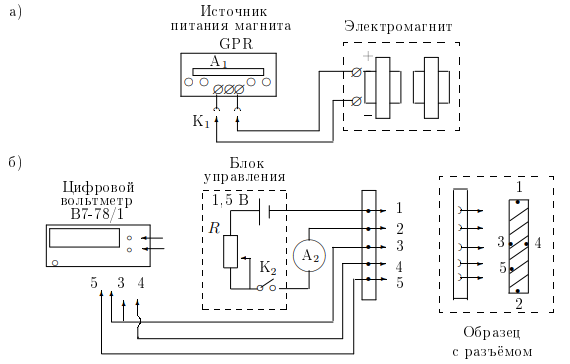
\includegraphics[width=12cm]{images/setup.png}
    \caption{Схема экспериментальной установки}
\end{figure}

\section*{Обработка результатов}
\indent Построим калибровочную кривую $B(I_1)$, чтобы пересчитывать по ней силу тока на величину магнитного поля.\ref{table:calibrovka}
\begin{table}[h!]
    \centering
    \begin{tabular}{|c|c|c|c|c|c|c|c|}
        \hline
        $I_1$, А & 0.3 \pm 0.01 & 0.6 \pm 0.01 & 0.9 \pm 0.01 & 1.2 \pm 0.01 & 1.5 \pm 0.01 & 1.8 \pm 0.01 & 2.1 \pm 0.01\\\hline
        $B$, Тл & 253\pm 1 & 493\pm 1 & 720\pm 1 & 933\pm 1 & 1093\pm 1 & 1173\pm 1 & 1240 \pm 1\\\hline
    \end{tabular}
    \caption{Зависимость поля внутри электромагнита от силы тока в нем}
\end{table}

\indent Теперь, измерив ЭДС Холла, построим семейство характеристик $\varepsilon_X = f(B)$ при разных значениях тока $I_2$ через образец. По ним определим коэффициенты наклона $K(I_2) = \Delta\varepsilon / \Delta B$.
\begin{table}[h!]
    \centering
    \begin{tabular}{|c|c|c|c|c|c|c|c|}
        \hline
        $U$, мкВ / $I_1$, А & 0.3 \pm 0.01 & 0.6 \pm 0.01 & 0.9 \pm 0.01 & 1.2 \pm 0.01 & 1.5 \pm 0.01 & 1.8 \pm 0.01 & 2.1 \pm 0.01\\\hline
        $I_2 = 0.3$ мА&-1.24& -0.17& 0.55& 1.22& 1.63& 1.90& 2.08\\\hline
        $I_2 = 0.4$ мА&-1.75& -0.35& 0.63& 1.44& 2.01& 2.4& 2.66\\\hline
        $I_2 = 0.5$ мА&-2.21& -0.41& 0.76& 1.74& 2.46& 2.93& 3.24 \\\hline
        $I_2 = 0.6$ мА&-2.76& -1.1& 0.86& 2.04& 2.9& 3.48& 3.83   \\\hline
        $I_2 = 0.7$ мА&-3.05& -0.7& 1.00& 2.29& 3.27& 3.92& 4.3   \\\hline
        $I_2 = 0.8$ мА&-3.62& -0.93& 1.04& 2.55& 3.68& 4.41& 4.85 \\\hline
        $I_2(\text{rev}) = 0.84$ мА&-12.39& -15.58& -18.11& -20.22& -21.5& -22.5& -23.04 \\\hline
    \end{tabular}
    \caption{Зависимость разности потенциалов $U$ от силы тока через источник питания магнита ($A_1$) при различных значениях силы тока через цепь ($A_2$)\\($\sigma_{U_{34}} = 0.002$ мВ; $\sigma_{U_2} = 0.005$ мA)}
\end{table}

\newpage
\begin{figure}[h!]
    \centering
    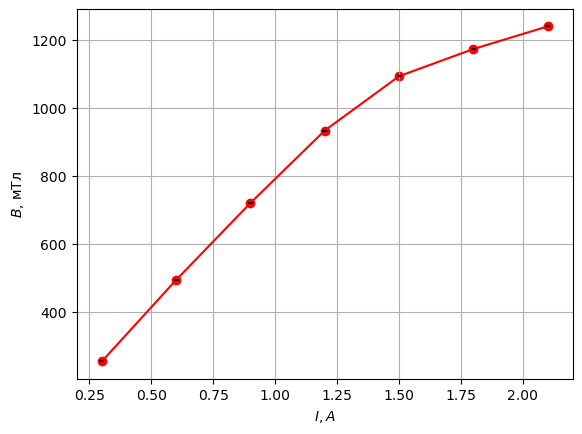
\includegraphics[width=13cm]{images/plot1.png}
    \caption{Зависимость индукции магнитного поля через электромагнит $B$ от силы тока $I_1$}
    \label{table:calibrovka}
\end{figure}

\begin{figure}[h!]
    \centering
    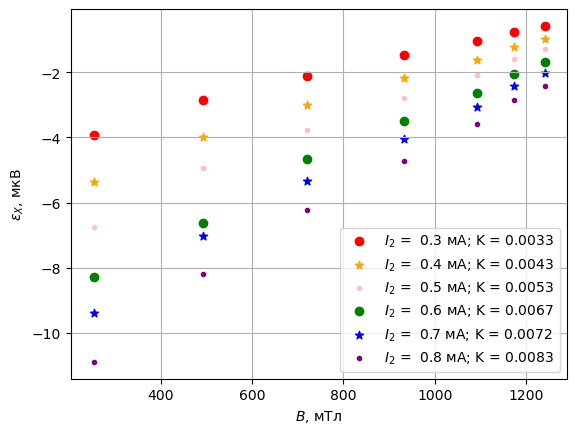
\includegraphics[width=14cm]{images/plot2.png}
    \caption{Зависимость ЭДС Холла $\varepsilon_X$ от магнитного поля $B$ при различных значениях силы тока через образец $I_2$}
    \label{table:mainplot}
\end{figure}
\newpage

\begin{table}[h!]
    \centering
    \begin{tabular}{|c|c|c|c|c|c|c|}
        \hline
        $I_2$, мА & 0.3 \pm 0.01 & 0.4 \pm 0.01 & 0.5 \pm 0.01 & 0.6 \pm 0.01 & 0.7 \pm 0.01 & 0.8 \pm 0.01\\\hline
        $K$, мкВ/Тл &3.3 \pm 0.2 & 4.3 \pm 0.2 & 5.3 \pm 0.3 & 6.7 \pm 0.4 & 7.2 \pm 0.4 & 8.3 \pm 0.5  \\\hline
    \end{tabular}
    \caption{Зависимость углового коэффициента $K$, гарфика зависимости ЭДС Холла от магнитного поля, от тока протекающего по образцу $I_2$}
\end{table}

\begin{figure}
    \centering
    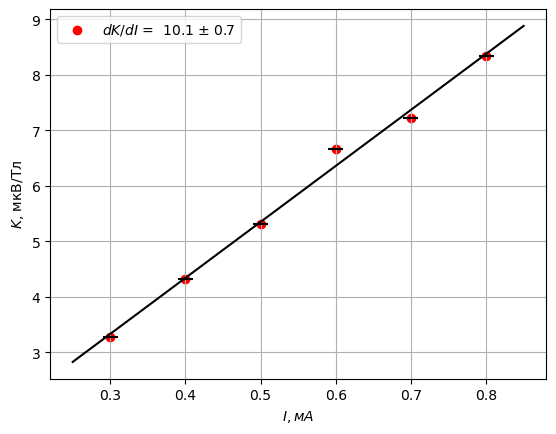
\includegraphics[width=14cm]{images/plot3.png}
    \caption{Зависимость углового коэффициента $K$, гарфика зависимости ЭДС Холла от магнитного поля, от тока протекающего по образцу $I_2$}
\end{figure}

\indent Для Холловского напряжения справедлива формула:
\begin{equation}
    \varepsilon_X = \frac{B}{nqh}\cdot I = R_H\cdot \frac{B}{a}\cdot I\label{eq:holl}
\end{equation}
\indent где $I$ - ток, протекающий через обазец; $R_H$ - постоянная Холла, знак которой определяется знаком заряда носителя.\\
\indent Тогда учитывая \ref{eq:holl} можем найти постоянную Холла и концентрацию носителей заряда в образце:
\begin{equation}
    R_H = \frac{dK}{dI} \cdot a = (2.0 \pm 0.1)\cdot 10^{-5} \text{ м}^3 / \text{Кл}
\end{equation}
\begin{equation}
n = \frac{1}{R_H q} = (3.1 \pm 0.2) \cdot 10^{23} \text{ м}^{-3}
\end{equation}
\indent Теперь рассчитаем удельную проводимость материала образца при напряжении \\$U_{35} = 0.13\pm 0.005$ мВ и токе через образец $I = 0.84\pm 0.005$ мА:
\begin{equation}
    \sigma =\frac {I\cdot L_{35}}{U_{35}\cdot a \cdot l} = (6.057 \pm 0.009)\cdot 10^3 \text{ См/м}
\end{equation}
\indent Теперь вычислим подвижность $b$ носителей тока:
\begin{equation}
    b = \frac{\sigma}{q n} = (1.2\pm 0.08)\cdot 10^{3}\text{ см}^2/ \text{В}\cdot\text{c}
\end{equation}

\begin{table}[h!]
    \centering
    \begin{tabular}{|c|c|c|c|c|}
        \hline
        $R_H$, м$^3$/Кл $\cdot 10^{-5}$ & Носители заряда & $n$, м$^{-3}$ & $\sigma $, См/м & $b$, см$^2$/В$\cdot$с \cdot $10^{3}$\\\hline
        2.0 \pm 0.1 & Дырки & (3.1\pm0.2)$\cdot 10^{23}$ & (6.057\pm 0.009)\cdot 10^3 & 1.2\pm 0.08\\\hline
        -  & - & - & 10^4 & 1.8\\\hline
    \end{tabular}
    \caption{Результаты измерений и сравнение их с табличными данными}\label{table:res}
    
\end{table}

\section*{Выводы}
\indent Определили носителей заряда в образце легированного германия - дырки, а так же вычислили их подвижность и концентрацию. Вычислили удельную проводимость образца. Результаты приведены в таблице \ref{table:res}.



\end{document}
